\subsection{Hub}

El flujo de datos empleado en este patrón de diseño ha sido inspirado en cómo se comunican los diferentes elementos en un servidor. Es decir, cualquier módulo del MVC deberá realizar una petición al servidor (Hub) y este se encargará de solventar y dar servicio a dicha petición. Se puede ver con mayor claridad cómo funciona y su implementación en la siguiente figura:\bigskip

\begin{figure}[!h]
    \centering
    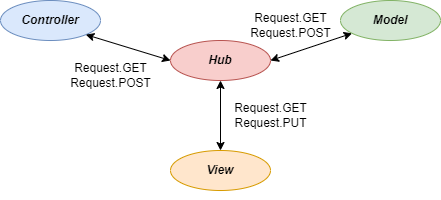
\includegraphics[width=\linewidth]{MVC/img/flujocom.png}
    \caption{Patrón MVC usado en la práctica.}
    \label{fig:flujo_datos}
\end{figure}

El Servidor/Hub se encarga de administrar los diferentes tipos de peticiones que llegan de los diferentes componentes. En la figura \ref{fig:flujo_datos} se observan los diferentes tipos de peticiones posibles que se pueden realizar, en concreto: GET, POST y PUT. En un entorno web, GET sirve para obtener datos, POST para enviar y PUT para actualizar. En el programa los diferentes tipos de peticiones se han traducido en: \medskip

\begin{description}
    \item[GET  ] Realiza un retorno del dato solicitado.
    \item[POST] Añade un el dato enviado.
    \item[PUT  ] Realiza un set del dato enviado.
\end{description}\medskip

Para permitir esta implementación, se ha creado la interfaz \texttt{Notify} con el método \texttt{notifyRequest} el cual deberá estar implementado en todos los módulos del MVC, ya que será el responsable de gestionar las peticiones y asegurar que cada uno de ellos puede realizar sus tareas designadas de manera eficiente y precisa.
